
% Table generated by Excel2LaTeX from sheet 'acronym'
\begin{table}[htbp]
	\centering
	%\begin{adjustwidth}{-0.2cm}{}
	\scriptsize
	\caption{Alphabetic list of acronyms used in this study.}
	\begin{tabular}{|L{2cm}|L{13cm}|}
		\hline
		\multicolumn{1}{|c|}{Acronym} & \multicolumn{1}{c|}{Usage} \\
		\hline
		23S.E & A biological rRNA dataset  \\
		\hline
		23S.E.aa\_ag & A biological rRNA dataset  \\
		\hline
		BBXY0MN & MN$^{th}$ BAliBASE instance under RVXY group \\
		\hline
		Clustal $\Omega$ & A state-of-the-art MSA method \\
		\hline
		Clustal W & A state-of-the-art MSA method \\
		\hline
		FN rate & False negative rate, measures quality of a phylogenetic tree w.r.t. the reference tree \\
		\hline
		FSA   & A state-of-the-art MSA method \\
		\hline
		Gap   & No. of gaps, an objective function that measures goodness of an MSA \\
		\hline
		GapCon & Concentration of gaps, an objective function that measures goodness of an MSA \\
		\hline
		Kalign & A state-of-the-art MSA method \\
		\hline
		MAFFT & A state-of-the-art MSA method \\
		\hline
		ML & Maximum likelihood approach for inferring a phylogenetic tree from an MSA\\
		\hline
		MSA   & Multiple sequence alignment \\
		\hline
		MUSCLE & A state-of-the-art MSA method \\
		\hline
		NSGA-II & A multi-objective metaheuristics  \\
		\hline
		NSGA-III & A multi-objective metaheuristics which an improved version of NSGA-II to handle more than three objective functions  \\
		\hline
		PASTA & A state-of-the-art MSA method \\
		\hline
		PRANK & A state-of-the-art MSA method \\
		\hline
		ProbCons & A state-of-the-art MSA method \\
		\hline
		R0   & A random replicate of 100-taxon simulated dataset \\
		\hline
		R14   & A random replicate of 100-taxon simulated dataset \\
		\hline
		R19   & A random replicate of 100-taxon simulated dataset \\
		\hline
		R4   & A random replicate of 100-taxon simulated dataset \\
		\hline
		R9   & A random replicate of 100-taxon simulated dataset \\
		\hline
		RetAlign & A state-of-the-art MSA method \\
		\hline
		RV11  & One of the six groups of BAliBASE 3.0 benchmark \\
		\hline
		RV12  & One of the six groups of BAliBASE 3.0 benchmark \\
		\hline
		RV20  & One of the six groups of BAliBASE 3.0 benchmark \\
		\hline
		RV30  & One of the six groups of BAliBASE 3.0 benchmark \\
		\hline
		RV40  & One of the six groups of BAliBASE 3.0 benchmark \\
		\hline
		RV50  & One of the six groups of BAliBASE 3.0 benchmark \\
		\hline
		SimG  & Similarity based on gap columns, an objective function that measures goodness of an MSA \\
		\hline
		SimNG & similarity based on non-gap columns, an objective function that measures goodness of an MSA \\
		\hline
		SOP   & Sum of pairs, an objective function that measures goodness of an MSA without using the reference alignment\\
		\hline
		SP score & Sum-of-pair score, measures quality of an MSA w.r.t. the reference alignment  \\
		\hline
		T-Coffee & A state-of-the-art MSA methods \\
		\hline
		TC & No. of totally aligned columns, an objective function that measures goodness of an MSA without using the reference alignment \\
		\hline
		TC score & Total-column score, measures quality of an MSA w.r.t. the reference alignment  \\
		\hline
		wSOP  & Weighted sum of pairs, an objective function that measures goodness of an MSA \\
		\hline
	\end{tabular}%
	\label{tab:acronyms}%
	%\end{adjustwidth}
\end{table}%

\section{Objective functions for MSA}
\label{sec:objective _function}
There are numerous objective functions defined for MSA in the literature. We identify the following widely used objective functions from the recent works and briefly discuss their feasibility in MSA:

\begin{itemize}
	
	\item \textbf{Maximize sum of pairs score}~\cite{seeluangsawat2005multiple, da2010alineaga}:  
	This is an extension of pairwise sequence alignment score. Pairwise score is calculated for each pair of aligned sequences. Then, we calculate the total score by summing pairwise scores of all possible pairs. In Figure \ref{fig:pairwise}, the pairwise score is calculated by considering the elements of the same columns of two aligned sequences with the scoring or substitution matrix $\delta$. There are some standard substitution matrices for biological sequences at~\url{ftp://ftp.ncbi.nih.gov/blast/matrices/}.
	
	
	\begin{figure}[!htbp]
		\begin{adjustwidth}{-0.2cm}{}
			\centering
			\begin{subfigure}[b]{0.5\columnwidth}
				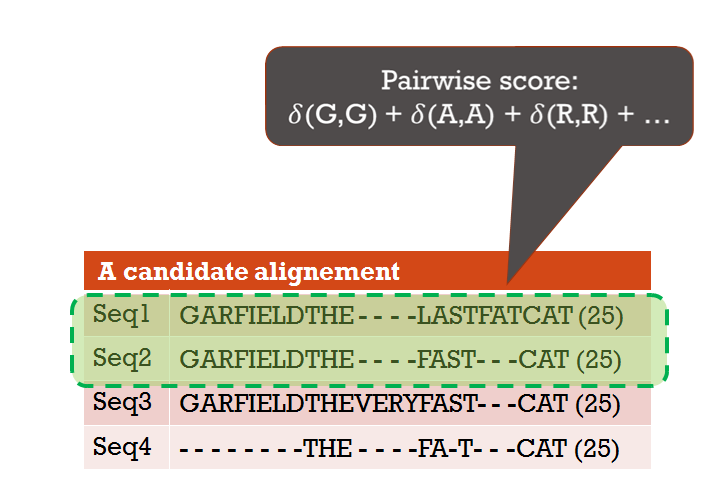
\includegraphics[width=\columnwidth]{Figure/pairwise}
				\caption{Pairwise score of two aligned sequences.}
				\label{fig:pairwise}
			\end{subfigure}	
			\begin{subfigure}[b]{0.5\columnwidth}
				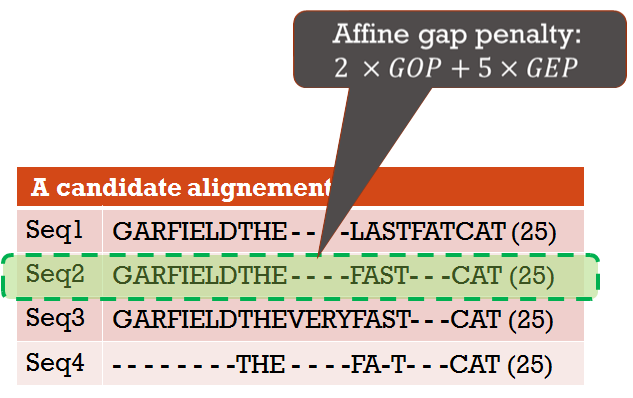
\includegraphics[width=\columnwidth]{Figure/agp}
				\caption{Affine gap penalty of an aligned sequence.}
				\label{fig:agp}
			\end{subfigure}
			\begin{subfigure}[b]{0.5\columnwidth}
				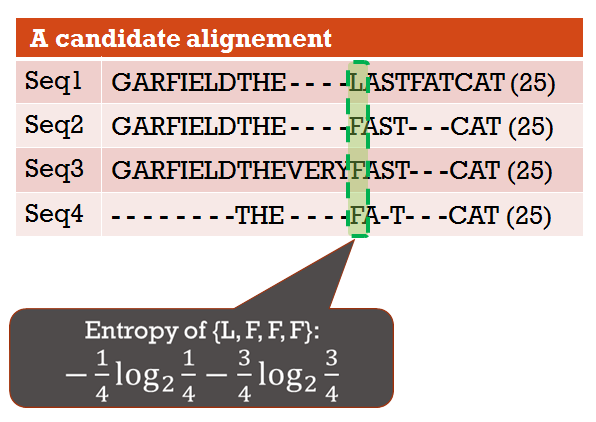
\includegraphics[width=\columnwidth]{Figure/entropy_score}
				\caption{Entropy of a column of alignment.}
				\label{fig:entropy}
			\end{subfigure}
		\end{adjustwidth}
		\caption{Three objective functions for MSA. The example alignment is adopted from~\citep{rubio2016hybrid}.}
		\label{fig:msa_obj}
	\end{figure}
	
	\item \textbf{Minimize entropy}~\cite{soto2014multi}: 
	Entropy is a measurement of dissimilarity in the same columns of different aligned sequences. When all the columns contain same element, the entropy is minimum \(0\). Again, the entropy is maximum \(1\) when every element is different. Total entropy is calculated by summing up entropy values of all columns. Figure \ref{fig:entropy} demonstrates the calculation of entropy for a single column. The problem with this function is that, while calculating entropy researchers treat gap as a separate character without proper justification.
	
	\item \textbf{Minimize affine gap penalty}~\cite{seeluangsawat2005multiple, kaya2014multiple, zhu2016novel, rani2016multiple}: 
	Affine gap penalty assigns different penalty for opening a gap ($GapOpeningPenalty, GOP$) and extending a gap ($GapExtension\-Penaly, GEP$) while computing gap penalty for a particular sequence. Then finally, summation of gap penalties of all sequences is to be minimized. An example is demonstrated in Figure \ref{fig:agp} showing the calculation of gap penalty of one sequence. Here two ideas (i.e. percentage of gap and concentration of gap) are combined without explanation. Also researchers face trouble to fix the value of two penalties.
	
	\item \textbf{Maximize weighted sum of pairs score with affine gap penalties}~\cite{rubio2016hybrid, rubio2016bee}:  
	Here two objectives are combined in the form: weighted sum of pairs score - affine gap penalty. To calculate weighted sum of pairs score, score of each pair of characters are multiplied by the sequence weight between that the corresponding two sequences. This weight is computed using the Levenshtein distance between two non-aligned sequences. Levenshtein distance is the is the minimum number of insertions, deletions or substitutions needed to convert one sequence into the other. 
	
	\item \textbf{Maximize number of totally aligned columns}~\cite{ortuno2013optimizing, da2010alineaga, rubio2016hybrid, rubio2016bee, ortuno2013optimizing, zambrano2017comparing}:
	Maximizing the number of totally aligned columns is the most simple used objective. But for input data comprising large number of taxa, its value is confined to a few values.
	
	\item \textbf{Minimize percentage of gaps}~\cite{abbasi2015local, ortuno2013optimizing, zambrano2017comparing}:
	High percentage of gaps means the sequences had to be significantly modified to align with each other. This is used as a minimizing objective function to find a better candidate solution. It can be also considered as percentage of non-gaps.
	
	\item \textbf{Maximize similarity}~\cite{kaya2014multiple, rani2016multiple}:
	%Similarity performs a measure of structural similarity among all sequences defining an individual. 
	For each column of MSA, similarity considers the ratio of the dominant character. This ratio is averaged over all columns. The closer the value of similarity is to one, the larger the probability that the candidate alignment will be discovered as the best possible alignment. Here we find similar problem as with entropy. Researchers discard gap while calculating ratio of characters in a column without sound reasoning. 
	
\end{itemize}

%\section{Multi-objective optimization}
\section{Multi-objective metaheuristics}
\label{sec:mop}
While optimizing multiple objective functions simultaneously, a multi-objective metaheuristics determines a set of solutions (instead of a single solution) which represents the best-possible compromise of all objectives. A solution is said to dominate another one if and only if it is equal to that solution in all objectives and also better than that in at least one objective. A solution is said to be Pareto optimal if no other solutions can dominate it. The set of all Pareto optimal solutions is called Pareto set and the image of pareto set in the objective space is known as Pareto front. However, practically a multi-objective metaheuristics aims to approximate the Pareto front as precisely as possible with a finite number of solutions.

%\subsection{Evolutionary algorithms}
Among metaheuristics, multi-objective evolutionary algorithms (MOEAs) are well-suited to solve multi-objective optimization problems~\cite{yang2013grid}. MOEAs deal with a set of possible solutions (known as population) at once which allows finding several members of the Pareto front in a single run of the algorithm. Moreover, they are  black-box optimization methods which do not need particular assumptions like continuity or differentiability of the decision space. 

%So the goal of a multi-objective metaheuristics is to output a set of solutions instead of a single solution., evolutionary algorithms (EAs) are population-based, They are well suited for multi-objective optimization. 

\begin{algorithm}[!htb]
	\caption{A General structure of MOEA}
	\begin{algorithmic}[1]\label{alg:MaOEA}
		\STATE{Randomly generate the initial population $ P_0 $}
		\STATE{Evaluate the objective functions of each individual in $ P_0 $}
		\STATE{$t \leftarrow 0$}
		\WHILE{$t <$ maximum value of $t$} 
		\STATE{Generate offspring population $ Q_t $ by applying \textit{Crossover} and \textit{Mutation} on $ P_t $}
		\STATE{Evaluate the objective functions of each individual in $ Q_t $}
		\STATE{Produce generation $ P_{t+1} $ from $ P_t $ and $ Q_t $ using \textit{Ranking scheme}}
		\STATE{$t \leftarrow t + 1$ }
		\ENDWHILE
	\end{algorithmic}
\end{algorithm}

A general structure of MOEAs is summarized in Algorithm \ref{alg:MaOEA}. Here the \textit{Crossover} and \textit{Mutation} are popularly known as genetic operators. They generate offspring (new solutions) from parents (existing solutions). These are problem-specific and designed based on the actual problem to be solved. \textit{Ranking scheme} is used to choose appropriate solutions to form the next generation. This is problem-independent concept and provided by the developers of a specific algorithm. In this study, we considered the three widely used MOEAs for multi-objective optimization. We briefly describe them as follows.

\begin{enumerate}[label=(\alph*)]
	
	\item NSGA-II~\citep{deb2002fast} follows the classical structure of a generational genetic algorithm. At first, it applies the typical genetic operators (selection, crossover, and mutation) on the current population to fill an auxiliary population. Then it builds the next-generation by incorporating the best individuals from both the current and auxiliary populations according to a Pareto ranking and the crowding distance operator. Perhaps it is the most commonly used algorithm for solving optimization problems having two or three objective functions. 
	
	\item NSGA-III~\citep{deb2014evolutionary} is designed to handle a large number of objective functions. The skeleton of NSGA-III remains similar to its predecessor NSGA-II with notable changes in its selection mechanism. At each generation, it produces an offspring population from the current population by applying genetic operators. These two populations are merged to form a new population using the selection mechanism. NSGA-III continues to use Pareto dominance as the primary selection criterion to promote convergence. But it substitutes the crowding distance operator in NSGA-II with a clustering operator aided by a set of well-distributed reference points as the secondary selection criterion to maintain diversity. NSGA-III has been shown to perform reasonably.
	%NSGAIII has been shown to perform reasonably on handling a large number of objective functions~\cite{deb2014evolutionary}.
	
	\item MOEA/D~\citep{zhang2007moea} is a representative decomposition based MOEA. Unlike Pareto dominance based methods (e.g., NSGA-II, NSGA-III), It decomposes the original problem into many single-objective subproblems using an aggregation function and a series of weight vectors defining the relative importance of different objectives. %We use the Das and Dennis's procedure~\cite{das1998normal} for generating uniform weight vectors, which are evenly distributed along the 7-dimensional unit hyper-plane. 
	Then it deals with these subproblems in a collaborative manner. Neighborhood relations among these subproblems are defined based on the similarity between their weight vectors. 
	%When optimizing a subproblem, the local information from its neighboring subproblems is shared. 
	Each subproblem maintains an individual which could be the best individual found so far for it. The algorithm generates a new individual for each subproblem by performing genetic operators on some of its neighboring individuals. The current individual of both the considered subproblem and its neighbors will be updated if the new individual is better than their current one. %The procedure of MOEA/D for TNDP is presented in Algorithm~\ref{alg:moead}.	(i.e., the individuals of its neighboring subproblems) that combines all objectives
	For MSA, we adopt the MOEA/D configuration used by~\citep{zhu2015novel}.  
\end{enumerate} 

We implemented the above two metaheuristics using jMetalMSA~\citep{zambrano2017multi} which is a Java metaheuristic framework for MSA. The important parameters with corresponding values are listed in Table~\ref{tab:parameters}. We adopt the same mutation and crossover operator, along with the associated parameter values, used by~\cite{ortuno2013optimizing}.  

\begin{comment}
We provide a short description of these operators below. 
%publicly available at~\url{https://github.com/jMetal/jMetalMSA}. 

\begin{itemize}
	
	\item The mutation operator is termed as closed gap shifting, where consecutive gaps are randomly chosen and shifted to another random position in a sequence. This shifting may result columns having only gaps which are then removed. Thus this mutation tries to reduce the number of gaps in the MSA. 
	
	\item The crossover operator is the single-point crossover over alignments proposed by~\citealp{da2010alineaga}. The operator randomly selects a column from one parent to split it into two blocks (let us refer to them P1a and P1b). The same selected positions are located in the other parent (which are not necessarily in the same column) and is tailored so that the right piece can be joined to the left piece of the first parent and vice versa (P2a and P2b). Finally, the selected blocks are exchanged between these two parents to create two new individuals with the combination of the blocks: [P1a + P2b] and [P1a + P1b]. After that, any empty space that appears at the junction point is filled with gaps.
	%NSGAIII has been shown to perform reasonably on handling a large number of objective functions~\cite{deb2014evolutionary}.	
\end{itemize}
\end{comment}

% Table generated by Excel2LaTeX from sheet 'param'
\begin{table}[!htbp]
	\centering
	\small
	\caption{Major parameters of our algorithms.}
	\begin{tabular}{|c|c|c|} %|c|C{3cm}|C{3.2cm}|
		\hline
		Algo. & \multicolumn{1}{c|}{Parameter} & Value \\
		\hline
		\multirow{5}{*}{All} & Max. generations & 500 \\
		
		\cline{2-3}          & Mutation  & Closed gap shifting \\
		\cline{2-3}          & Mutation rate & 0.2 \\
		\cline{2-3}          & Crossover  & Single-point crossover \\
		\cline{2-3}          & Crossover rate & 0.8 \\ %, $C_r$
		\hline
		\multirow{2}{*}{NSGA-II} & Population size & 100 \\ %, $\overline{N}$
		\cline{2-3}          & No. of runs & 20 \\
		\hline
		\multirow{3}{*}{NSGA-III} & No. of reference points & 120 \\
		\cline{2-3}          & Population size & 120 (78) \\ %, $N$
		\cline{2-3}          & No. of runs & 25 (40) \\
		\hline
		\multirow{2}{*}{MOEA/D} & Population size & 100 \\ %, $\overline{N}$
		\cline{2-3}          & No. of runs & 20 \\
		\cline{2-3}          & Neighborhood size & 10 \\
		\cline{2-3}          & Aggregation function & Tchebycheff approach \\
		\hline
	\end{tabular}%
	\label{tab:parameters}%
\end{table}%

%\subsection{Our multi-objective metaheuristic framework}
%\label{sec:mof}
% Table generated by Excel2LaTeX from sheet 'multi-pc'

\begin{comment}
\subsubsection{Solution Initialization}
Instead of initializing solutions randomly, which is the usual practice in metaheuristics, we seed the initial population with alignments generated by nine state-of-the-art MSA tools. These tools are listed in Table~\ref{tab:msa_tools}. We create the required number of initial solutions by randomly mixing and modifying those nine alignments. 
%Among these tools PASTA is the most recently developed. Due to its simultaneous estimation of alignment and phylogenetic tree, it is expected to be the most robust.

\begin{table*}[htbp]
\small
\centering
\caption{List of state-of-the-art MSA tools that we used initialize the metaheuristics.}
\begin{tabular}{|l|l||l|l|}
\hline
\multicolumn{2}{|c||}{For nucleotide sequences} & \multicolumn{2}{c|}{For protein sequences} \\
\hline
\multicolumn{1}{|c|}{Tool} & \multicolumn{1}{c||}{Version} & \multicolumn{1}{c|}{Tool} & \multicolumn{1}{c|}{Version} \\
\hline
FSA~\citep{bradley2009fast} & 1.15.9 & FSA   & 1.15.9 \\
\hline
PASTA~\citep{mirarab2015pasta} & 1.7.8 & PASTA & 1.7.8 \\
\hline
T-Coffee~\citep{notredame2000t} & 11.00 & T-Coffee & 11.00 \\
\hline
MAFFT~\citep{katoh2002mafft} & 7.31  & MAFFT & 7.245 \\
\hline
Clustal W~\citep{thompson1994clustal} & 2.1   & Clustal W & 2.1 \\
\hline
Clustal $ \Omega $~\citep{sievers2011fast} & 1.2.4 & RetAlign~\citep{szabo2010reticular} & 1.0 \\
\hline
MUSCLE~\citep{edgar2004muscle} & 3.8.31 & MUSCLE & 3.8.31 \\
\hline
PRANK~\citep{loytynoja2005algorithm} & 0.170427 & ProbCons~\citep{do2005probcons} & 1.12 \\
\hline
Kalign~\citep{lassmann2008kalign2} & 2.03  & Kalign & 2.04 \\
\hline
\end{tabular}%
\label{tab:msa_tools}%
\end{table*}%

\subsubsection{Genetic Operator}
Both of our metaheuristics used the same genetic operator (i.e. mutation and crossover), which were used by~\citealp{ortuno2013optimizing}. \citealp{zambrano2017multi} illustrated their functions. Here we provide a short description of these operators. 

The mutation operator is termed as closed gap shifting, where consecutive gaps are randomly chosen and shifted to another random position in a sequence. This shifting may result columns having only gaps which are then removed. Thus this mutation tries to reduce the number of gaps in the MSA.

The crossover operator is the single-point crossover over alignments proposed by~\citealp{da2010alineaga}. The operator randomly selects a column from one parent to split it into two blocks (let us refer to them P1a and P1b). The same selected positions are located in the other parent (which are not necessarily in the same column) and is tailored so that the right piece can be joined to the left piece of the first parent and vice versa (P2a and P2b). Finally, the selected blocks are exchanged between these two parents to create two new individuals with the combination of the blocks: [P1a + P2b] and [P1a + P1b]. After that, any empty space that appears at the junction point is filled with gaps.
%\subsubsection{Multi-objective evolutionary algorithm}
%\subsubsection{Parameter Configuration}
\end{comment}

\begin{comment}


\section{Evaluation of estimated alignments}
\label{sec:msa_eval}
We evaluate estimated alignments with respect to reference alignment using two well-known alignment quality scores called TC score and SP score. These two scores are defined below:
\begin{itemize}
	\item TC score is the ratio of the number of correctly aligned columns in the estimated alignment to the total number of aligned columns in the reference alignment. This is also known as column score.
	
	\item SP score is the ratio of the number of aligned pairs in the estimated alignment to the total number of aligned pairs in the reference alignment.
	
	%\item Pairs score is the mean of SP-score and Modeler. SP-Score is the ratio of the number of aligned pairs to the total number of aligned pairs in the reference alignment. And Modeler is very similar to the SP-score where we take the ratio of the number of aligned pairs to the total number of aligned pairs in the estimated alignment  	
\end{itemize}
For both the measures, higher value implies better score.

\section{Phylogenetic tree estimation}
\label{sec:tree_estimation}
For each of the generated alignment we estimate the phylogenetic tree using Maximum Likelihood (ML) method which is the standard way of estimating phylogenetic tree from sequence data~\cite{liu2011raxml}. FastTree\citep{price2010fasttree} and RAxML~\citep{stamatakis2014raxml} are the most widely used software for this purpose. FastTree can produce output very quickly with little (and in some cases no) degradation in tree accuracy, as compared to RAxML~\cite{liu2011raxml}. In this study we had to estimate a large number of phylogenetic trees. So we choose FastTree over RAxML.
%We used a popular tool named FastTree-2 developed by \citep{price2010fasttree}. %It is publicly available at \url{http://www.microbesonline.org/fasttree/}.

\section{Evaluation of phylogenetic tree}
\label{sec:tree_eval}
We evaluate the quality of each estimated ML tree with respect to the true phylogenetic tree using a widely used measure known as the False Negative (FN) rate. FN rate is the percentage of edges present in the true tree but missing in the estimated tree. So a small value of FN rate is desirable. Although there are two more common tree error measures (False Positive (FP rate) and and Robinson-Foulds (RF) rate), all of them are identical when true and estimated trees are binary~\citep{warnow2017computational}. In this study we worked with binary trees only. %as a quality measure, 

\section{Evaluation of objective functions}
\label{sec:obj_eval}
In the context of phylogeny estimation, a desired objective function for MSA should lead to such alignments which can produce highly accurate (having small FN rate) ML trees. Considering this fact, we try to evaluate the effectiveness of an objective function by studying how its values are associated with the corresponding FN rates. The objective function that frequently exhibits positive correlation with FN rate is predicted to be a good optimization criteria. To accomplish this, we fit multiple linear regression model to calculate the degree of association (i.e., regression coefficient) between an objective and FN rate. Then we apply t-test, with null hypothesis that there is no association, to check the significance of individual regression coefficients. It should be noted that, such regression results does not necessarily indicate the strength of an objective as an optimization criterion. However, such results can definitely be utilized as the starting point for experimentation for further validation.

\end{comment}